
\subsection{Instrumenting the IDE -- Building it Yourself for Visual Studio} 
\label{buildItYourself}

This section is a tutorial sequence of exercises that support student projects for implemeting a personal monitoring tool for Visual Studio.  Each exercise allows the student to discover technical aspects of monitorning tools in a way that builds capabilities towards a monitoring tool.  Readers attempting the tutorial should be familiar with the .NET event model used to manage GUI commands in .NET applications, have demonstrated capability programming in C sharp, and have working knowledge of Visual Studio.  

The goal is to build a Visual Studio Extension that collects key command events from Visual Studio that generate the Navigation Ratio metric (See \ref{BuildingDataCollection} for each day's development activity.  The extension will startup when Visual Studio starts, automatically collect events from the IDE, and save the data to a local file.  For simplicity, the extension will not perform any background processing thus the user may notice a delay on Visual Studio startup due to this exension's setup process.  The first time the extension runs, it will create a configuration file that allows the user to specifiy which events it will record and how it will classify those events as structured or unstructured navigation.  The extension will create a new time-stamped log file each time it starts and record the events for that execution of Visual Studio in the log file. 


 \begin{Exercise}[type={program}, difficulty={1}]
\begin{enumerate}
\item
The first step in instrumenting Visual Stuidio is to create a Visual Studio Extension that creates a log file when it starts.   Microsoft provides a project creation wizard for generating a Visual Stuido extension (called a Package) when you install the Visual Studio SDK.  So first install the Visual Studio SDK.  

\item Create a new project in C sharp selecting Extensibility and Visual Studio Package under the new project creation dialog as shown in figure \ref{fig:ProjectCreation}.  
\begin{figure}
	\centering
	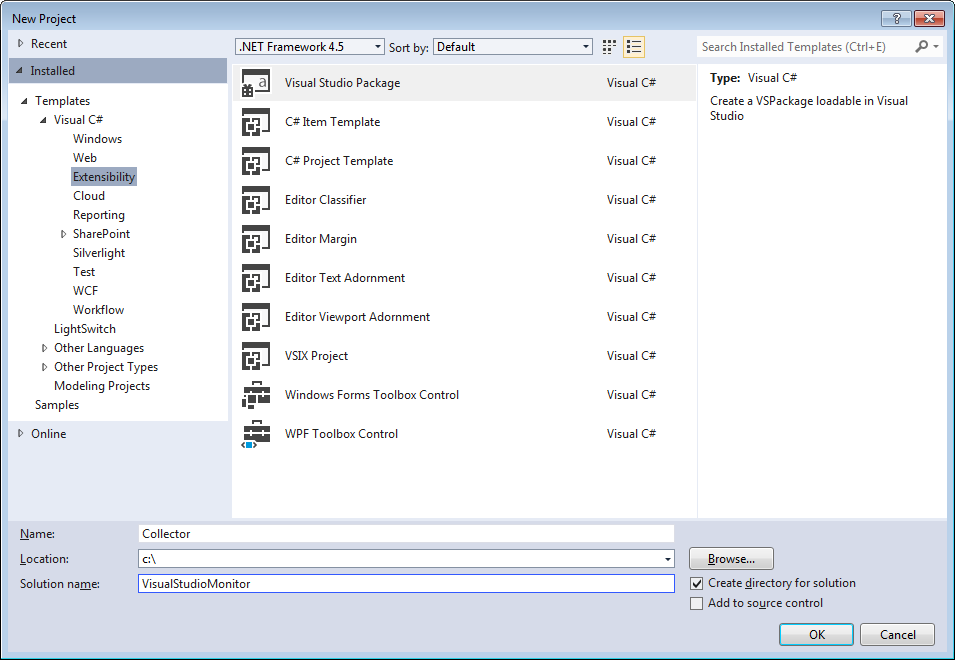
\includegraphics[width=4in]{Graphics/CreateVSIXExtension.png}
	\caption{Create a Visual Studio Extension}
	\label{fig:ProjectCreation}
\end{figure}

Give the project and solution a name and follow the default options for each step of the wizard.  When asked to specify what type of extension, click only the option to generate a menu command.  In the following step, give the menu command a name of "Stop Monitoring" and a command ID of "StopCollector".  This menu option will allow the user to halt collection of data if they wish without quitting Visual Studio.  
\end{enumerate}
\end{Exercise}

 \begin{Answer}

\begin{enumerate}
\item
After creating the project and solution, the solution explorer should look like figure \ref{fig:SolutionExplorer} showing the project files necessary for the extension to work.
\begin{figure}
	\centering
	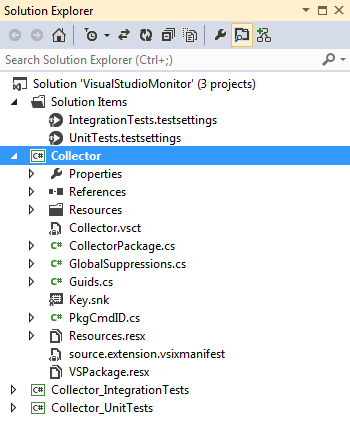
\includegraphics[width=2.5in]{Graphics/SolutionExplorer.png}
	\caption{Solution Explorer with Visual Studio Extension}
	\label{fig:SolutionExplorer}
\end{figure}
\end{enumerate}
\end{Answer}

\begin{Exercise}[type={program}, difficulty={1}]
\begin{enumerate}
\item
Good practice in extension development is to create a separate project (dll) for logic specific to the extension.  Add a class library type project to  the "Monitor" solution provide the data collection from Visual Studio and call it "Monitor".
\item
The next step is to create a static class that will manage the log file including starting, stopping recording data, and inserting data into the log file.  We will call this class "DataRecorder".   
Create a "DataRecorder" Class in the Collector project.  Because we don't want more than one recorder running at a time and want to access this class without instantiating it, make the class static.  Have the DataRecorder write a message to the file whenever it starts and stops.
\item
Finally, insert a call to DataMonitor.Start() at the end of the Initialize() method in the CollectorPackage class.  This will start the monitoring each time Visual Studio starts.  You will need to add a reference for the "Monitor" project to the Collector project, sign the Monitor project (you can use the snk file generated when the solution was created in step 1), then rebuild the solution.
\end{enumerate}
\end{Exercise}


\begin{Answer}

The call to DataRecorder.Start() is inserted in the CollectorPackage as shown in Listing \ref{code:StartCall}.
\begin{lstlisting}[caption=Call to DataRecorder.Start(),label=code:StartCall]
        /////////////////////////////////////////////////////////////////////////////
        // Overridden Package Implementation
        #region Package Members

        /// <summary>
        /// Initialization of the package; this method is called right after the package is sited, so this is the place
        /// where you can put all the initialization code that rely on services provided by VisualStudio.
        /// </summary>
        protected override void Initialize()
        {
            Debug.WriteLine (string.Format(CultureInfo.CurrentCulture, "Entering Initialize() of: {0}", this.ToString()));
            base.Initialize();

            // Add our command handlers for menu (commands must exist in the .vsct file)
            OleMenuCommandService mcs = GetService(typeof(IMenuCommandService)) as OleMenuCommandService;
            if ( null != mcs )
            {
                // Create the command for the menu item.
                CommandID menuCommandID = new CommandID(GuidList.guidCollectorCmdSet, (int)PkgCmdIDList.StopCollector);
                MenuCommand menuItem = new MenuCommand(MenuItemCallback, menuCommandID );
                mcs.AddCommand( menuItem );
            }
            DataRecorder.Start();
        }
        #endregion
\end{lstlisting}

The source code for the DataRecorder.cs file is shown in Listing \ref{code:DataRecorder}
\begin{lstlisting}[caption=Data Recorder Class,  label=code:DataRecorder]
using System;
using System.Collections.Generic;
using System.Linq;
using System.Text;
using System.Threading.Tasks;

namespace Monitor
{
    public static class DataRecorder
    {
        public static void Start() {
            logDirectoryPath = System.IO.Path.GetTempPath();
            logFileName = System.IO.Path.Combine(logDirectoryPath, "collector " + DateTime.Now.ToString("yyyy-MM-dd HH.mm.ss") + ".log");
            try {
                using (System.IO.StreamWriter streamWriter = new System.IO.StreamWriter(
                    new System.IO.FileStream(logFileName, System.IO.FileMode.OpenOrCreate, System.IO.FileAccess.Write, System.IO.FileShare.ReadWrite)
                    ))
                {
                    streamWriter.WriteLine("Collector Started");
                }
            } 
            catch (System.IO.IOException ioexception) {
                Console.WriteLine("Error creating log file "+ioexception);
            }
         }

        public static void Stop() {

                WriteLog("Collector Stopped");
            
        
        }

        public static void WriteLog(string logToWrite)
        {
            try
            {
                using (System.IO.StreamWriter streamWriter = new System.IO.StreamWriter(
                    new System.IO.FileStream(logFileName, System.IO.FileMode.Append, System.IO.FileAccess.Write, System.IO.FileShare.ReadWrite)
                    ))
                {
                    streamWriter.WriteLine(logToWrite);
                }
            }
            catch (System.IO.IOException ioexception)
            {
                Console.WriteLine("Error writing to log file " + ioexception);
            }
        
        }

        private static string logFileName;
        private static string logDirectoryPath;
    }
}

\end{lstlisting}
\end{Answer}


\newpage
Visual Studio processes all command events through the DTE object that also provides the API for extending Visual Studio.  Command events are any command that the user performs in the IDE using a menu, shortcut button, or quick launch command. This step builds a class to query Visual Studio for all the supported commands in the IDE and store them in a file for annotation and later use.  

\begin{enumerate}
\item

 Fortunately the DTE object has a query method that lists all the commands it manages.   The DTE query method is Commands that returns an IEnumerable collection of EnvDTE.Command objects.  You will need to get a reference to the DTE object and then process the Commands object results in a loop.  Listing below provides a method to try to get a reference to the DTE.  It depends on references to EnvDTE, Microsoft.VisualStudio.Shell.12.0, and Microsoft.VisualStudio.OLE.Interop.  

%\begin{lstlisting}[caption=Method to get a DTE Reference,label=code:tryGetDTEObject,float=ht]
\begin{lstlisting}

		using EnvDTE;
		using Microsoft.VisualStudio.Shell; //12.0
		private static DTE tryGetDTEObject()
		{
			DTE dteobj=null;
			try
			{
				dteobj = ((EnvDTE.DTE)ServiceProvider.GlobalProvider.GetService(typeof(EnvDTE.DTE).GUID)).DTE;

			}
			catch (NullReferenceException)
			{}
			//Important to catch the following exception if the DTE object is unavailable
			catch (System.Runtime.InteropServices.InvalidComObjectException)
			{} 
			//Important to catch the following exception if the DTE object is busy
			catch (System.Runtime.InteropServices.COMException)
			{}
			return dteobj;
		}

\end{lstlisting}

\item
The EnvDTE.Command object contains fields for Guid (a GUID string), ID and integer sub-id, Name a readable name for the command.  To register an event handler for a EnvDTE.Command, you need get an object reference for the command using the Guid and ID to identify the command. The Name is useful information to understand what the command is.    There are several versions of the DTE object corresponding to versions of Visual Studio.  Depending on the commands of interest, each version may need to be queried for its commands.  

\end{enumerate}


 \begin{Exercise}[ type={program}, difficulty={1}]

In this step, build the classes required to query the DTE for all commands and store them for later use preferably in a text or XML format file.  You will need an extra field to allow you to select or classify the command to be monitored.  Call the method(s) to query and store from the Start() method from the DataRecorder class in the previous exercise so that the Monitor will save the commands on startup.
Recommended design pattern for this exercise is a Simple Factory pattern.  With this pattern an abstract base class provides common definitions for class fields that will be used for monitoring different Visual Studio events, conversion of those fields to and from the storage format, and (eventually) calling the WriteLine method in the recorder when the event fires.  The concrete creator class is the class specific to Visual Studio commands that manages the fields available from the DTE.Command class.  The client in the Simple Factory pattern is a class that maintains the collection of events that either gets read from the file or queried from Visual Studio.
\end{Exercise}

\begin{Answer}
The previous exercise adds a feature to query the DTE and save the commands to a file.  The instruction hinted that more than one class may be used, though the implementation could take place without class members that hold the DTE Command attributes.  The following class design provides the ability to store and retrieve command attributes and anticipates other types of monitored events outside the scope of commands.

The AbstractMonitoredEvent class in listing %\ref{code:AbstractMonitoredEvent}
 provides an abstraction of what data and methods are needed to setup event monitoring in VisualStudio.  Initially the class only deals with data that we save about the event, later it will include methods and parameters used to register the event and capture its invocation.

%\lstinputlisting[caption=Abstract Monitored Event, label=code:AbstractMonitoredEvent,   float=h]{c:/VisualStudioMonitor/Monitor/AbstractMonitoredEvent.cs}

The MonitoredCommandEvent in listing %\ref{code:MonitoredCommandEvent}
makes the AbstractMonitoredEvent class concrete for Visual Studio commands.  It implements a constructor that builds a MonitoredCommandEvent object from the Command class of the DTE or a constructor that builds from an XElement.  An output method ToXElement translates the object to XML for saving.
%\lstinputlisting[caption=MonitoredCommandEvent,  label=code:MonitoredCommandEvent,  float=h]{c:/VisualStudioMonitor/Monitor/MonitoredCommandEvent.cs}

The MonitoredEventFactory in listing %\ref{code:MonitoredEventFactory}
 is a static class that completes our Simple Abstract Factory pattern provding the methods to create an object inheriting from AbstractMonitoredEvent from an XElement or a Command object.  
%\lstinputlisting[caption=MonitoredEventFactory,  label=code:MonitoredEventFactory,  float=h]{c:/VisualStudioMonitor/Monitor/MonitoredEventFactory.cs}

The MonitoredEventCollection in listing %ref{code:MonitoredEventCollection}
 is the Client in our pattern that maintains a "stock" of all the monitored events we need to manage.  It currently provides methods to read MonitoredEvents from a file, save them to a file, and query them from the Visual Studio DTE.  Events are managed in a List object belonging to this class.   The constructor initializes the List object from a configuration file if the file exists, otherwise it initializes the List object from the Visual Studio DTE's Command object and saves the List to the configuration file. 
%\lstinputlisting[caption=MonitoredEventCollection,  label=code:MonitoredEventCollection,  float=h]{c:/VisualStudioMonitor/Monitor/MonitoredEventCollection.cs}

\end{Answer}

\begin{Exercise}
The previous exercise adds a feature to query the DTE and save the commands to a file.  In this step we will add the ability to read that file and register event processing to save each command invocation to a log file.   The classes we need to define are already part of the project based on the design from the previous step.  We extend the AbstractMonitoredEvent class to add virtual methods that handle registering and de-registering (on dispose), and a virtual method for writing to the log.  Each concrete implementation of Abstract MonitoredEvent must override these methods, add an object of the type of event monitored, and an event handler to process the event data and write to the log.  

Registering for DTE events is the process of inserting an event handler for each command of interest into the event notification structure of the DTE.  Starting with AbstractMonitoredEvent class, create a virtual method to register events with the DTE.  This method accepts a DTE object as a parameter and returns a boolean if the registration takes place.

\begin{lstlisting}
public virtual bool RegisterEventForMonitoring(DTE dteobject) {

	if (!isDisposed) {
	
	}
}
\end{lstlisting}

The next method is a non-virtual and a virtual Dispose method with a boolean argument of the current disposing state.  The methods take care of disconnecting the event handler when the class exits and possibly more importantly, control a boolean that prevents registration from taking place when the object is waiting for finalization.

\begin{lstlisting}
protected bool isDisposed;

public void Dispose() {
	this.Dispose(true);
}

protected virtual void Dispose(bool disposing) {
	//In here take care of disconnecting the event handler after checking the disposing state
	this.isDisposed=true;
}
\end{lstlisting}

Finally, place a non-virtual To-Log method that will unify the log output for all derived classes.  ToLog can call the WriteLog method of the DataRecorder class created in a previous exercise.

Now that the abstract class is ready, a walkthrough of the MonitoredCommandEvent class is in order.  The class needs a field of the class EnvDTE.CommandEvents to store the specific DTE command monitored in each instance of a MonitoredCommandEvent.  Then it is time to override the virtual RegisterEventForMonitoring method using this field and the DTE.  Registering first must find the event in the DTE and assign it to the field, then attach a new event hander to the event.  The following code performs the finding and assignment:

\begin{lstlisting}
private CommandEvents eventTypeObject;

public override bool RegisterEventForMonitoring(DTE dte)
{
    if (!isDisposed && eventTypeObject == null && dte != null)
    {
    		//this finds the event based on Guid and EventID combined
        eventTypeObject = dte.Events.get_CommandEvents(Guid, EventID) as CommandEvents;
    }
		
}
\end{lstlisting}

Now to attach an event handler, simply add an event handler "OnAfterExecute"' to the established event object as follows:
\begin{lstlisting}
if (eventTypeObject != null) 
	eventTypeObject.AfterExecute += new _dispCommandEvents_AfterExecuteEventHandler(OnAfterExecute);
return (eventTypeObject != null);
\end{lstlisting}              

Use the Visual Studio "Generate" command to generate a method stub for OnAfterExecute and the
code will compile.  Place a call to log the event information in the OnAfterExecute event handler.

\end{Exercise}

\begin{Answer}
The exercise provided a detailed step-by-step approach for this part of the work.  Listings for AbstractMonitoredEvent and CommandMonitoredEvent are below.

%\lstinputlisting[caption=AbstractMonitoredEvent,  label=code:AbstractMonitoredEvent,  float=h]{c:/VisualStudioMonitor/Monitor/AbstractMonitoredEvent.cs}

%\lstinputlisting[caption=MonitoredCommandEvent,  label=code:MonitoredCommandEvent,  float=h]{c:/VisualStudioMonitor/Monitor/MonitoredCommandEvent.cs}

\end{Answer}

 summary:
\begin{enumerate}
	\item 
	Identify the goal (or research questions) and metrics for measurement that requires IDE data.  express attributes of the goal such as how time should be measured, how events should be classified or grouped, and derived calculations.
	\item
	Identifying  IDE API interfaces necessary to accomplish the measurement goal.  Examples window showing events, scrolling in the editor, clicking on code lines, Command events, automated events (e.g. build begin and end).
	\item
	The event interceptor model, intercepting IDE events transparently to the user.  consider Throttling the capture of near real-time events such as scrolling.
	\item
	Considerations for anonymizing the collected data
	\item
	IDE data collection tooling.  Build tooling for ease of use and installation.  Planning logging interface for offline and online data collection.  Handling data store access.  Ways to address security.  
	\item
	End user communication including anonymity, statement of intended use, restrictions on use, optional participation
	
\end{enumerate}
